


\section{Pre-training}
\begin{figure}[t]
    \centering
    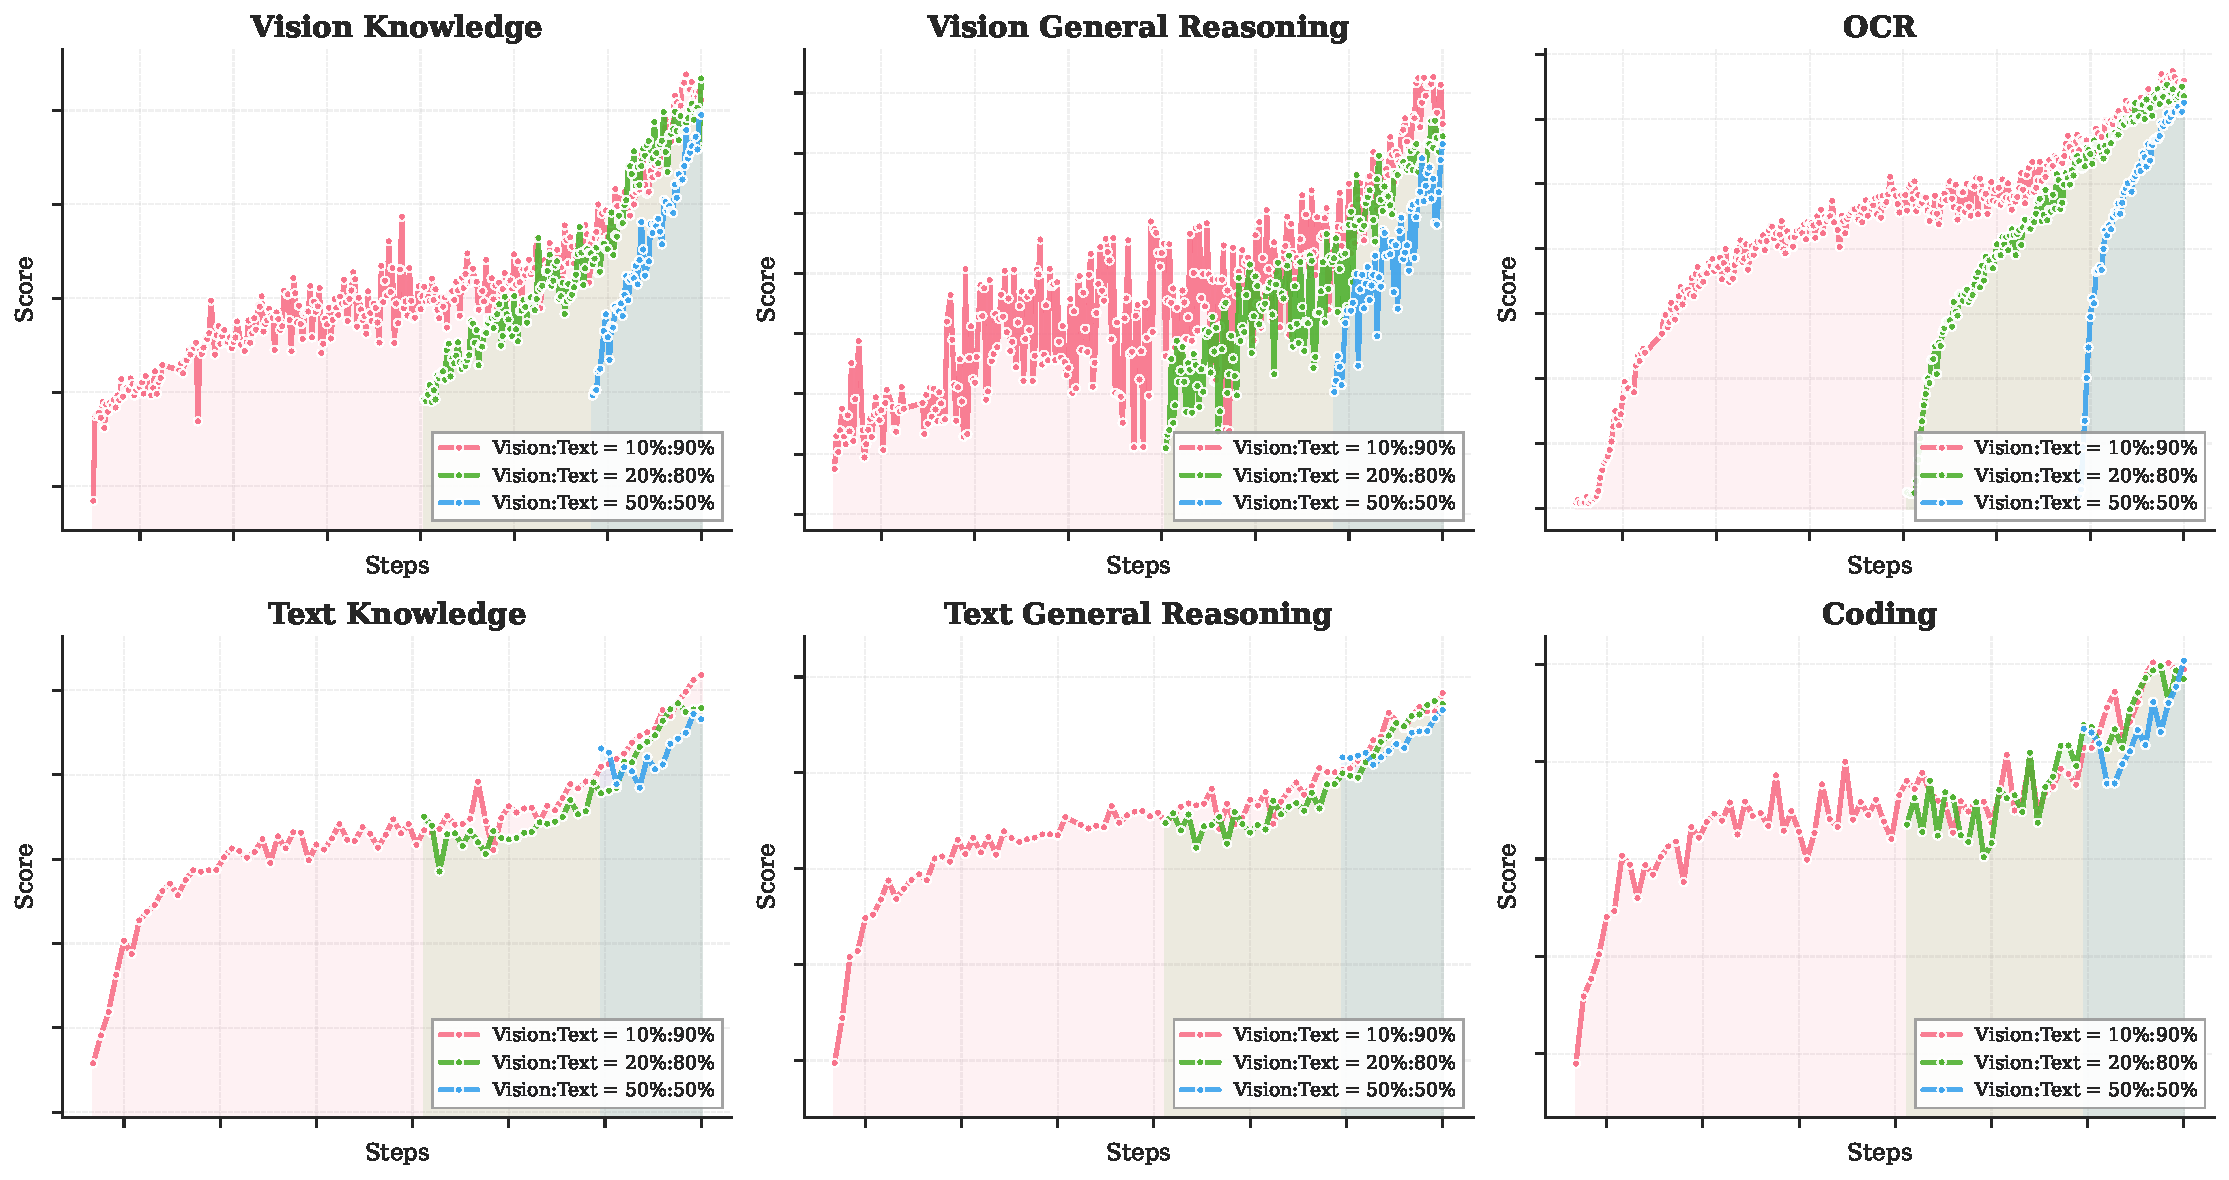
\includegraphics[width=\textwidth]{figures/vision-joint.pdf}
    \caption{Learning curves comparing vision-to-text ratios (10:90, 20:80, 50:50) under fixed vision-text token budget across vision and language tasks. Early fusion with lower vision ratios tend to yield better results.} 
    \label{fig:joint-train}
\end{figure}

\subsection{Joint-Training}
We further provide the full training curves for all configurations in Figure~\ref{fig:joint-train}. Notably, we observe a "dip-and-recover" pattern in text performance during mid-fusion and late-fusion stages: when vision data is first introduced, text capability initially degrades before gradually recovering. We attribute this to the modality domain shift—the sudden introduction of vision tokens disrupts the established linguistic representation space, forcing the model to temporarily sacrifice text-specific competence for cross-modal alignment.

In contrast, early fusion maintains a healthier and more stable text performance curve throughout training. By co-optimizing vision and language from the outset, the model naturally evolves unified multimodal representations without the shock of late-stage domain migration. This suggests that early exposure not only prevents the representation collapse observed in late fusion but also facilitates smoother gradient landscapes for both modalities. Collectively, these findings reinforce our proposal of native multimodal pre-training: moderate vision ratios combined with early fusion yield superior convergence properties and more robust bi-modal competence under fixed token budgets.

\subsection{Text data}
The Kimi K2.5 pre-training text corpus comprises curated, high-quality data spanning four primary domains: Web Text, Code, Mathematics, and Knowledge. Most data processing pipelines follow the methodologies outlined in Kimi K2~\citep{team2025kimik2}. For each domain, we performed rigorous correctness and quality validation and designed targeted data experiments to ensure the curated dataset achieved both high diversity and effectiveness.

\textbf{Enhanced Code Intelligence}
We upweighted code-centric data, significantly expanding (1) repository-level code supporting cross-file reasoning and architectural understanding, (2) issues, code reviews and commit histories from the internet capturing real-world development patterns, and (3) code-related documents retrieved from PDF and webtext corpora. These efforts strengthen repository-level comprehension for complex coding tasks, improve performance on agentic coding subtasks such as patch generation and unit test writing, and enhance code-related knowledge capabilities.

\subsection{Vision data}
Our multimodal pre-training corpus includes seven categories: caption, interleaving, OCR, knowledge, perception, video, and agent data. Caption data~\citep{schuhmann2022laion, gadre2024datacomp} provides fundamental modality alignment, with strict limits on synthetic captions to mitigate hallucination. Image-text interleaving data from books, web pages, and tutorials~\citep{zhu2024multimodal,laurenccon2024obelics} enables multi-image comprehension and longer context learning. OCR data spans multilingual text, dense layouts, and multi-page documents. Knowledge data incorporates academic materials processed via layout parsers to develop visual reasoning capabilities.

Furthermore, we curate a specialized multimodal problem-solving corpus to bolster reasoning within Science, Technology, Engineering, and Mathematics domains. This data is aggregated through targeted retrieval and web crawling; for informational content lacking explicit query formats, we employ in-context learning~\citep{brown2020languagemodelsfewshotlearners} to automatically reformulate raw materials into structured academic problems spanning K-12 to university levels. To bridge the modality gap between visual layouts and code data, we incorporate extensive image-code paired data. This includes a diverse array of code formats—such as HTML, React, and SVG, among others—paired with their corresponding rendered screenshots, enabling the model to align abstract structural logic with concrete visual geometry.


For agentic and temporal understanding, we collect GUI screenshots and action trajectories across desktop, mobile, and web environments, including human-annotated demonstrations. Video data from diverse sources enables both hour-long video comprehension and fine-grained spatio-temporal perception. Additionally, we incorporate grounding data to enhance fine-grained visual localization, including perception annotations (bounding boxes), point-based references. We also introduce a new contour-level segmentation task~\citep{song2026pixellevelvlmperceptionsimple} for pixel-level perception learning. All data undergoes rigorous filtering, deduplication, and quality control to ensure high diversity and effectiveness.


\section{Infra}
Kimi K2.5 is trained on NVIDIA H800 GPU clusters with 8$\times$400 Gbps RoCE interconnects across nodes. We employ a flexible parallelism strategy combining 16-way Pipeline Parallelism (PP) with virtual stages~\citep{huang2019gpipeefficienttraininggiant,narayanan2021efficientlargescalelanguagemodel}, 16-way Expert Parallelism (EP)~\citep{lepikhin2020gshard}, and ZeRO-1 Data Parallelism, enabling training on any number of nodes that is a multiple of 32. EP all-to-all communication is overlapped with computation under interleaved 1F1B scheduling. To fit activations within GPU memory constraints, we apply selective recomputation for \texttt{LayerNorm}, \texttt{SwiGLU}, and \texttt{MLA} up-projections, compress insensitive activations to FP8-E4M3, and offload remaining activations to CPU with overlapped streaming.

\subsection{Data Storage and Loading}
We employ S3 \citep{amazon_s3} compatible object storage solutions from cloud providers to house our VLM datasets.
To bridge the gap between data preparation and model training, we retain visual data in its native format and have engineered a highly efficient and adaptable data loading infrastructure.
This infrastructure offers several critical advantages:
\begin{itemize}
\item \textbf{Flexibility:} Facilitates dynamic data shuffling, blending, tokenization, loss masking, and sequence packing throughout the training process, enabling adjustable data ratios as requirements evolve;
\item \textbf{Augmentation:} Allows for stochastic augmentation of both visual and textual modalities, while maintaining the integrity of 2D spatial coordinates and orientation metadata during geometric transformations;
\item \textbf{Determinism:} Guarantees fully deterministic training through meticulous management of random seeds and worker states, ensuring that any training interruption can be resumed seamlessly --- the data sequence after resumption remains identical to an uninterrupted run;
\item \textbf{Scalability:} Achieves superior data loading throughput via tiered caching mechanisms, robustly scaling to large distributed clusters while regulating request frequency to object storage within acceptable bounds.
\end{itemize}
Furthermore, to uphold uniform dataset quality standards, we have built a unified platform overseeing data registration, visualization, statistical analysis, cross-cloud synchronization, and lifecycle governance.